\chapter{The Large Hadron Collider and the ATLAS experiment}
\label{chap:ATLASdetector}

\chapterquote{Very inspiring quote}
{Very inspiring quote author}

%% LHC and ATLAS introduction
\section{The \LHC}
\label{sec:LHCandATLAS}

The massive fruit of labour, decades in the making from the hundreds of institutions which make up CERN, lies hidden 100 meters below the surface of the Switzerland-France border. Sandwiched between Geneva and the Jura Mountains is a 27 km ring of superconducting magnets and radio-frequency (RF) cavities, which bend and accelerate particles to 0.999999991$c$. Mathematically, this is approximately 3 metres per second slower than the speed of light. This remarkable achievement is none other than the Large Hadron Collider (LHC). The LHC lives up to its name; it is the largest machine built by humankind, and unsurprisingly the most powerful high-energy particle collider in the world. The four main interaction points around the ring where particles collide mark the four main experiments: ATLAS, CMS, LHCb, and ALICE. The former two are general purpose detectors with a similar goal: to precisely study the Standard Model and to search for evidence of new physics. The latter two have specialized purposes. LHCb is dedicated to probing physics involving b-hadrons in pp collisions, and ALICE’s aim is to shed light on the physics of the quark-gluon plasma by investigating heavy-ion collisions. 

Prior to the injection into the LHC, the protons first pass through a series of smaller machines which boost them to higher and higher energy. The first in the chain is LINAC2, a linear accelerator that spouts protons (the source of which is hydrogen atoms with electrons stripped away) at \unit{50}{\MeV}. Next the protons are piped into the Proton Synchrotron Booster, the Proton Synchrotron, and finally into the Super Proton Synchrotron \todo{Give more details about each of these steps}. Through this chain the protons get boosted to \unit{1.4}{\GeV} by the PSB, then further to \unit{25}{\GeV} by the PS, to a final \unit{450}{\GeV} by the SPS before entering the LHC. Inside the pipes of the LHC, the protons take a short 20 minutes to reach \unit{6.5}{\TeV}. 

\begin{figure}
  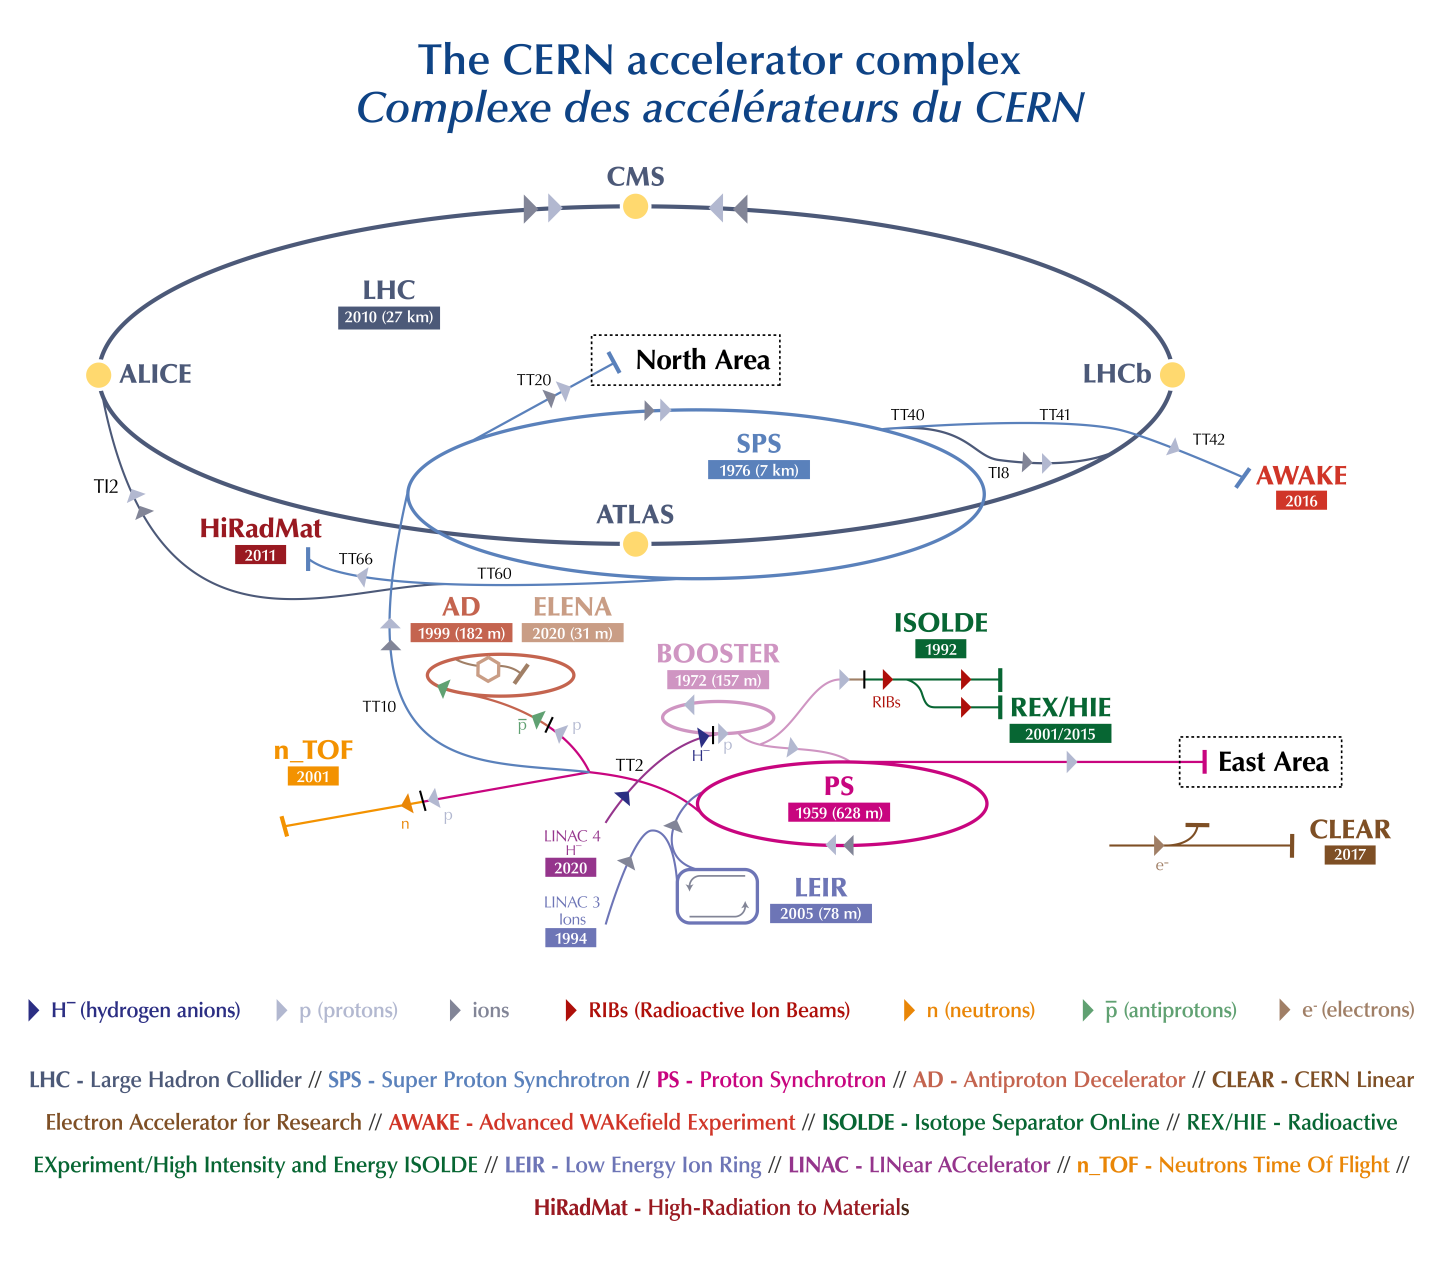
\includegraphics[width=\mediumfigwidth]{Figures/LHC/CernAcceleratorComplex.png}
  \caption[The \CERN accelerator complex]%
  {The CERN accelerator complex, where the LHC is the largest ring. The four main collision points corresponding to the main experiments are dotted in yellow.}
  \label{fig:CERNComplex}
\end{figure}

The impressive feat of accelerating particles is made possible through the use of radio-frequency cavities. The idea was first crafted by the young Rolf Wideröe \cite{vretenar2012radio} for his PhD thesis and later caught the eye of the brilliant E. Lawrence, recipient of the Nobel Prize in Physics in 1939 for the invention of the cyclotron. RF cavities are round chambers along the beam. A voltage generator generate a voltage which oscillates at \unit{400}{\mega\hertz}, inducing an electric field inside the RF cavity. As particles pass through they experience the force of the field and are accelerated along the beam pipe. In total the LHC uses 8 RF cavities per beam (so 16 in total), with each cavity capable of delivering a 2 megavolts (MV). Protons travelling through the cavity increase their energy to 14 times the injection amount, from 450 GeV to 6.5 TeV. Once protons get up to speed, a proton that has perfect timing will stay put, while protons that arrive slightly earlier/later will be accelerated/decelerate. The result is a beam of protons sorted into smaller segments of proton bunches. The LHC produces two such proton beams, one circulating clockwise and the other counterclockwise. 

An important key concept in particle physics is luminosity. It is a factor that relates the cross-section to the number of event per second, written as follows:
$$\luminosity=\dfrac{1}{\sigma}\cdot\dfrac{dN}{dt}$$
where \luminosity is the luminosity, $N$ is the number of events, and $\sigma$ is the production cross section. The dimension of luminosity is events per unit time and unit area \unit{}{\cm\rpsquared}\unit{}{\second\rp}.

There are two properties used to describe a particle beam: its \todo{write more about this} emittance $\epsilon$, and its $\beta$ function. The emittance can be thought of as the area occupied by the particle beam in the position momentum plane. A lower emittance means the distance between particles and the difference in momentum between the particles are small. The cross sectional sizes of the beam $\sigma_i$ ($i=x,y$) are written as 
$$\sigma_i=\sqrt{\dfrac{\beta_i\cdot\epsilon_i}{\pi}}$$ The beams are assumed to be Gaussian distributed, meaning that in collisions, the centres of the beams contribute most while the edges have minimal impact. Following this the luminosity is
$$\luminosity=\dfrac{N_1N_2f_{rev}N_b}{2\pi\Sigma_x\Sigma_y}$$
where $N_1$ and $N_2$ are the number of particles for each bunch, $N_b$ is the number of bunches, $f$ is the revolution frequency, and $\Sigma_x,\Sigma_y$ represent the \unsure{Erm what is a convolution..?} convolution of the beam sizes. They can be expressed as
$$\Sigma_x=\sqrt{\sigma_{x1}^2+\sigma_{x2}^2}, \quad \Sigma_y=\sqrt{\sigma_{y1}^2+\sigma_{y2}^2}.$$
Assuming that the beam sizes are identical and round, $\sigma_{x1}=\sigma_{x2}=\sigma_{y1}=\sigma_{y2}$, and the luminosity becomes
$$\luminosity=\dfrac{N_1N_2f_{rev}N_b}{4\pi\sigma^2}=\dfrac{N_1N_2f_{rev}N_b\gamma}{4\pi\epsilon_N\beta^*}.$$

When proton beams cross at the LHC, there are many collisions which occur other than the hard-scatter of interest. While increasing the number of particles per bunch increases the likelihood of a rare interaction, it also increases the pile-up of multiple interactions. Pile-up, denoted as $\mu$, is one of the biggest obstacles for LHC experiments; the more there is, the more difficult it becomes to disentangle the events of interest from the sea of low energy collision. It is, however, an inevitable consequence that accompanies increasing the instantaneous luminosity \todo{Write more about why int. lumi. is wanted to be high}. The contribution to pile-up events can be separated into two main categories: 
\begin{itemize}
  \item In-time pile-up refers to simultaneous proton-proton collisions occurring in the same bunch crossing as the hard scatter of interest;
  \item Out-of-time pile-up is the overlay of events from neighbouring bunches which contaminate signal events, attributed to detector electronics latency.
\end{itemize}
There are also less-substantial contributions from the cavern background, beam halo events, and beam gas events. The cavern background is the cloud of gas that floods the LHC cavern during operation. Beam halo events are from when the proton beam interacts with the collimating instrumentation, and the beam gas events describe interactions between the beam and the residual gas in the beam pipe. 

The \LHC was originally designed to reach a peak instantaneous luminosity and average pile-up of \unit{$10^{34}$}{\rpsquare{\cm}\reciprocal{\second}} and $\langle\mu\rangle=19$ respectively. 

\begin{figure}
  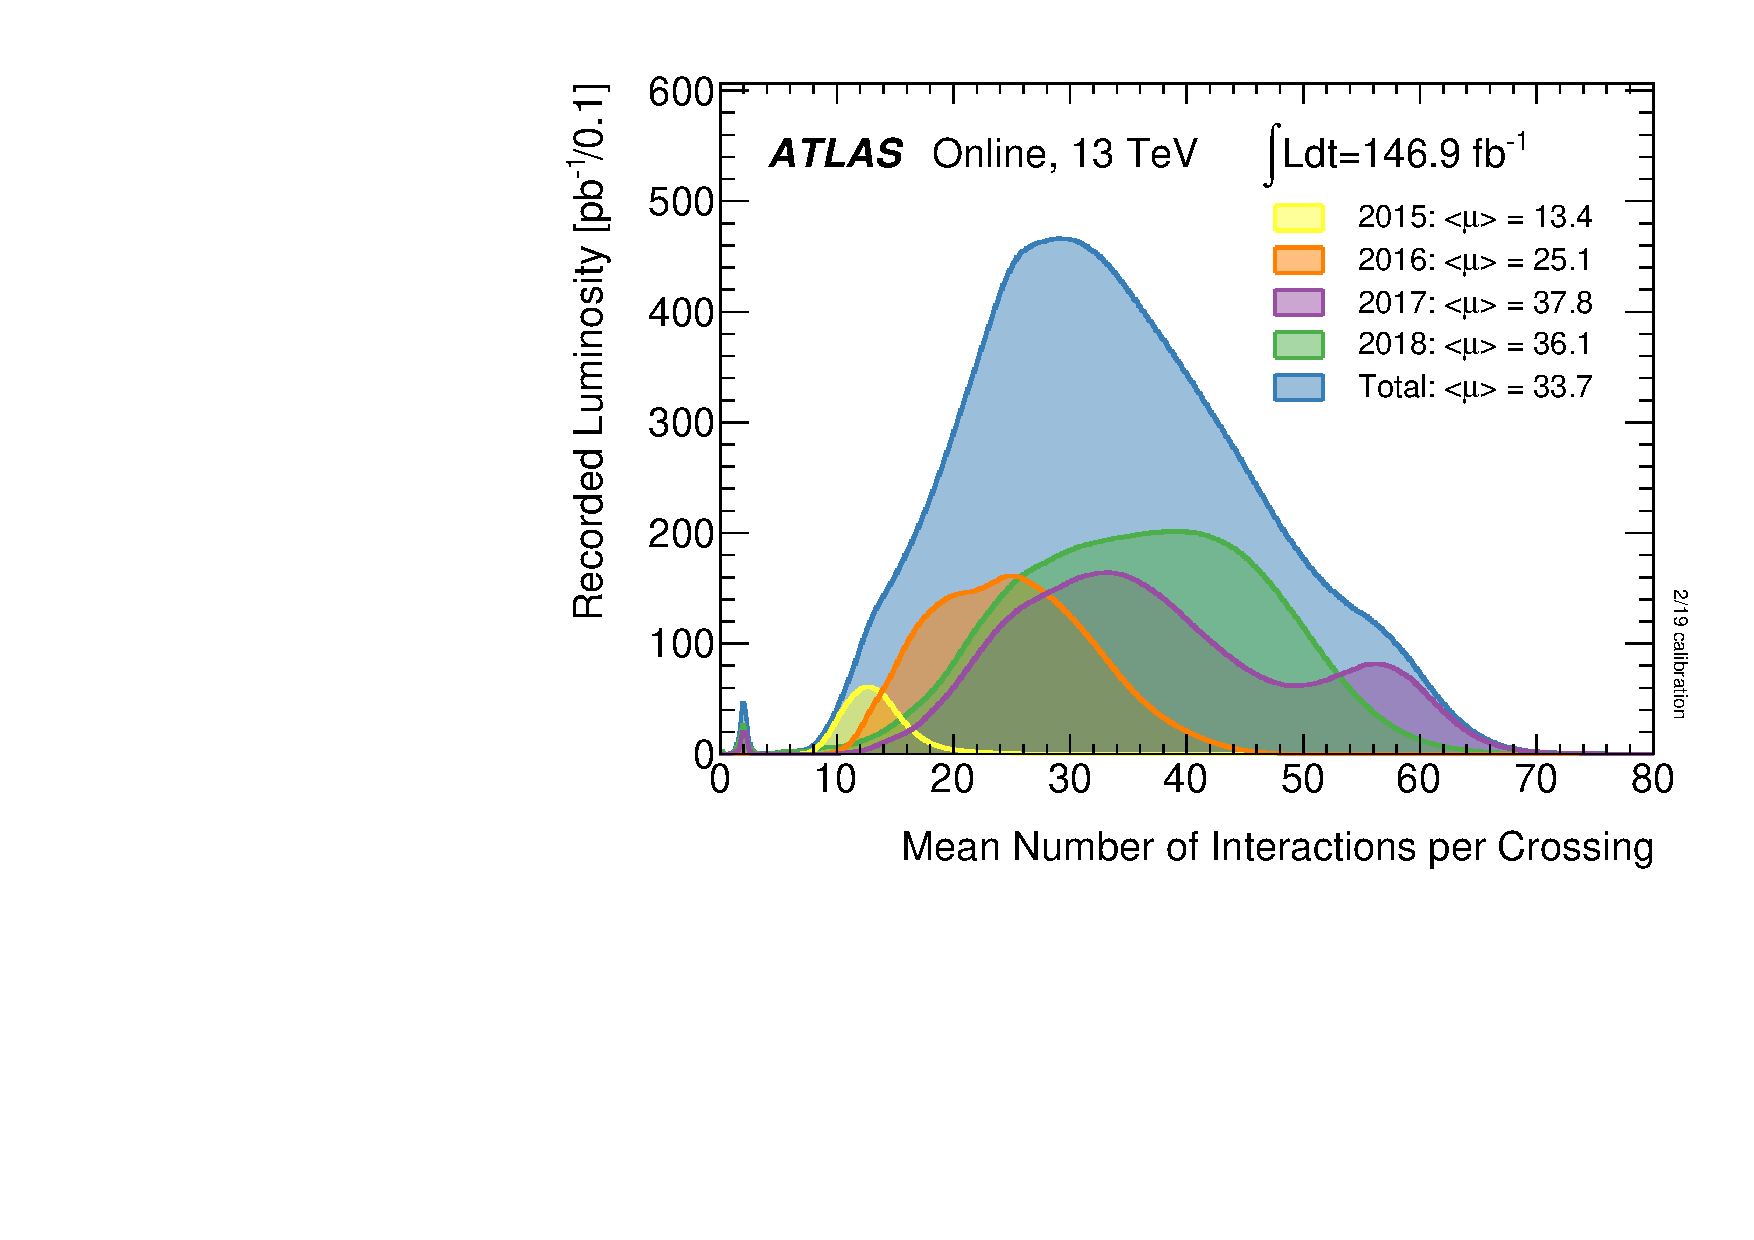
\includegraphics[width=\smallfigwidth]{Figures/LHC/PileUp_2015_2018.pdf}
  \caption[Pile-up distributions.]
  {The pile-up, $\mu$, is the mean number of collisions per bunch crossing. Shown is the \unit{13}{\TeV} are the pile-up distributions from 2015-2018, where each distribution is luminosity weighted.}
  \label{fig:Pileup}
\end{figure}
